\documentclass[final]{beamer}

% Use beamerposter with A0 portrait
\usepackage[size=a0,orientation=landscape,scale=1.01]{beamerposter}
% \usepackage[size=a0,orientation=portrait,scale=1.05]{beamerposter}

% Basic packages
\usepackage[utf8]{inputenc}
\usepackage[T1]{fontenc}
\usepackage{lmodern}
\usepackage{graphicx}
\usepackage{booktabs}
\usepackage{multicol}
\usepackage{wrapfig}
\usepackage{natbib}
\bibliographystyle{unsrtnat}

% \usepackage{enumitem} % REMOVED to avoid beamer conflict
\usepackage{hyperref}
\usepackage{array}
\usepackage{ragged2e}
\usepackage{colortbl}
\usepackage{xcolor}
\usepackage{etoolbox} % for safe list tweaks
\usepackage{microtype}
\usepackage{listings}
\usepackage[most]{tcolorbox}
\usepackage{tikz}
\usetikzlibrary{decorations.pathreplacing,calc,shadows}
\tcbuselibrary{skins,listings,breakable}

% Safer list spacing
\makeatletter
\patchcmd{\itemize}{\def\makelabel}{\setlength{\itemsep}{0.2em}\def\makelabel}{}{}%
\patchcmd{\enumerate}{\def\makelabel}{\setlength{\itemsep}{0.2em}\def\makelabel}{}{}%
\makeatother

% Colors
\definecolor{royal}{HTML}{0B132B}        % deep midnight blue
\definecolor{accent}{HTML}{F15152}       % vibrant coral
\definecolor{softbg}{HTML}{F7FAFC}       % airy background
\definecolor{mint}{HTML}{06AED5}         % bright aqua
\definecolor{highlight}{HTML}{FFC857}    % warm highlight
\definecolor{violet}{HTML}{5B2E90}       % punchy violet
\definecolor{danger}{HTML}{F46036}       % bold alert orange
\definecolor{columnblue}{HTML}{E6F6FA}   % column wash
\definecolor{datasetgreen}{HTML}{2CB978} % dataset tab green
\definecolor{codegreen}{HTML}{2CB978}
\definecolor{codeblue}{HTML}{0F8BCE}
\definecolor{codepurple}{HTML}{6C4AB6}
\definecolor{codeorange}{HTML}{F9A620}
\definecolor{codered}{HTML}{F15152}
\definecolor{codegray}{HTML}{6B7B8A}
\definecolor{codecomment}{HTML}{2F8F83}
\definecolor{codestring}{HTML}{E85D75}

\setbeamercolor{normal text}{fg=royal,bg=softbg}
\setbeamercolor{structure}{fg=mint}
\setbeamercolor{alerted text}{fg=danger}
\setbeamercolor{block title}{fg=white,bg=mint!80!royal}
\setbeamercolor{block body}{fg=royal,bg=white!96!softbg}
\setbeamercolor{block title alerted}{fg=white,bg=accent!80!danger}
\setbeamercolor{block body alerted}{fg=royal,bg=white!90!softbg}
\setbeamercolor{titlewrap}{fg=white,bg=royal}
\setbeamercolor{titleaccent}{fg=highlight,bg=royal}
\setbeamercolor{columnthreebox}{fg=royal,bg=columnblue}
\setbeamercolor{metriccardbox}{fg=royal,bg=white!96!mint}
\setbeamercolor{calloutbox}{fg=royal,bg=white!95!accent}

\lstdefinestyle{codestyle}{%
  backgroundcolor=\color{white},
  basicstyle=\ttfamily\small,
  keywordstyle=\color{codeblue}\bfseries,
  commentstyle=\color{codecomment}\itshape,
  stringstyle=\color{codestring},
  numberstyle=\scriptsize\color{codegray},
  numbers=left,
  numbersep=10pt,
  showstringspaces=false,
  breaklines=true,
  breakatwhitespace=true,
  tabsize=2,
  keepspaces=true,
  columns=fullflexible
}
\lstset{style=codestyle}

\newtcblisting{codeblock}[3][]{
  listing only,
  breakable,
  enhanced,
  colframe=#3,
  colback=#3!6!white,
  coltitle=#3!80!black,
  fonttitle=\bfseries\footnotesize,
  title={#2},
  arc=2mm,
  boxrule=0.5pt,
  left=2mm,
  right=2mm,
  top=2mm,
  bottom=2mm,
  attach boxed title to top left={yshift=-2mm,xshift=4mm},
  boxed title style={
    sharp corners,
    colframe=#3,
    colback=#3!18!white,
    boxrule=0.5pt
  },
  listing options={style=codestyle,#1}
}

\newenvironment{greencode}[2][]{
  \begin{codeblock}[#1]{#2}{codegreen}
}{\end{codeblock}}

\newenvironment{bluecode}[2][]{
  \begin{codeblock}[#1]{#2}{codeblue}
}{\end{codeblock}}

\newenvironment{purplecode}[2][]{
  \begin{codeblock}[#1]{#2}{codepurple}
}{\end{codeblock}}

\newenvironment{orangecode}[2][]{
  \begin{codeblock}[#1]{#2}{codeorange}
}{\end{codeblock}}

\newenvironment{redcode}[2][]{
  \begin{codeblock}[#1]{#2}{codered}
}{\end{codeblock}}

\newcommand{\datasetbox}[2]{%
  \tcbox[colframe=#2,colback=#2!88!white,boxrule=0pt,sharp corners,arc=0pt,left=6mm,right=6mm,top=2.6mm,bottom=2.6mm,fontupper=\small\bfseries\color{white}]{#1}%
}

\usefonttheme{professionalfonts}
\renewcommand{\familydefault}{\sfdefault}
\setbeamerfont{title}{series=\bfseries,family=\sffamily,shape=\upshape}
\setbeamerfont{block title}{series=\bfseries,family=\sffamily}
\setbeamerfont{block body}{family=\sffamily}
\setbeamerfont{section title}{series=\bfseries,family=\sffamily}
\setlength{\parskip}{0.26em}
\setlength{\parindent}{0pt}
\setlength{\columnsep}{2.0cm}
\setbeamertemplate{blocks}[rounded][shadow=true]
\newcommand{\key}[1]{\textbf{\color{accent}#1}}
\newcommand{\highlight}[1]{\textcolor{accent}{\textbf{#1}}}
\newcommand{\metriccard}[2]{%
  \begin{beamercolorbox}[wd=\linewidth,sep=0.8em,center,rounded=true,shadow=false]{metriccardbox}%
    {\Large\bfseries\color{accent}#1}\\[-0.25em]
    {\footnotesize #2}%
  \end{beamercolorbox}%
}
\newcommand{\callout}[2]{%
  \begin{beamercolorbox}[wd=\linewidth,sep=0.35em,rounded=true,shadow=false]{calloutbox}%
    {\bfseries\color{royal}#1}\\[-0.3em]
    {\small #2}%
  \end{beamercolorbox}%
}

% Paper size
% \setlength{\paperwidth}{841mm}
% \setlength{\paperheight}{1189mm}

\setbeamertemplate{background}{%
  \begin{tikzpicture}[remember picture,overlay]
    \path[fill=white] (current page.south west) rectangle (current page.north east);
    \shade[top color=softbg!95!white,bottom color=white] (current page.north west) rectangle (current page.south east);
    \path[fill=white,opacity=0.92] ($(current page.south west)+(2cm,2cm)$) rectangle ($(current page.north east)+(-2cm,-6cm)$);
  \end{tikzpicture}%
}

\title{\textbf{\huge Reconstruction of the Sunspot Number Series : Gathering Data}}
% \subtitle{Challenges and Benefits for the Space Climate Community}
\author{\texorpdfstring{\large \textcolor{highlight}{\textbf{Kalugodu Chandrashekhar}}\textsuperscript{1}, Laure Lef\`evre\textsuperscript{1}, Benjamin Mampaey\textsuperscript{1}, Senthamizh Pavai Valliappan\textsuperscript{1}, Hisashi Hayakawa\textsuperscript{2}, Christian Ritter\textsuperscript{3}}{\normalsize Chandrashekhar (1), Lefevre (1), Mampaey (1), Pavai Valliappan (1), Hayakawa (2), Ritter (3)}}
\institute{\texorpdfstring{\normalsize \textsuperscript{1} Royal Observatory of Belgium (ROB), \textsuperscript{2} Nagoya University, \textsuperscript{3} Universit\'e Catholique de Louvain, Louvain-la-Neuve, Belgium}{ROB; Nagoya; Universite Catholique de Louvain}}

% Logos (replace with your own files)
\newcommand{\leftlogo}{../logos/observatory_400x332.jpg}
\newcommand{\rightlogo}{../logos/silso-logo.png}
\newcommand{\farsunlogo}{../figures/ack_.png}
% \newcommand{\rightlogo}{../logos/BELSPO_1867x1563.jpg}

% Title box
\setbeamertemplate{headline}{%
  \leavevmode
  \begin{tikzpicture}[remember picture,overlay]
    \path[fill=royal] (current page.north west) rectangle ($(current page.north east)+(0,-8cm)$);
    \path[fill=accent!45!royal] ($(current page.north west)+(0,-0.15cm)$)
      .. controls +(8,-1.1) and +(-4,3.6) .. ($(current page.north)+(0,-3.2cm)$)
      .. controls +(4,-2.6) and +(-6,1) .. ($(current page.north west)+(0,-7cm)$);
    \path[fill=mint!45!royal,opacity=0.65] ($(current page.north east)+(-4cm,-0.45cm)$) circle (4.3cm);
    % Place left logo at the top-left of the header overlay
    \node[anchor=north west] at ($(current page.north west)+(0.8cm,-0.7cm)$) {%
      \includegraphics[height=3.4cm]{\leftlogo}
    };
  \end{tikzpicture}%
  \begin{beamercolorbox}[wd=\paperwidth,ht=7.4cm,dp=0ex,leftskip=1.8cm,rightskip=1.8cm]{titlewrap}
  \vspace{0.4cm}
    \begin{minipage}[t]{0.17\paperwidth}
      \vspace{0pt}
      \centering
      \includegraphics[height=4.1cm]{\leftlogo}
    \end{minipage}%
    \begin{minipage}[t]{0.53\paperwidth}
      \vspace{0pt}
      \raggedright
%      {\fontsize{60}{62}\selectfont \textbf{FAR\textcolor{accent}{Su}N}}\\[-0.1cm]
%      {\small \color{accent}\textbf{Findability and Accessibility of historical Raw Sunspot Numbers}}\\[0.25cm]
      {\color{white}\bfseries\fontsize{44}{46}\selectfont \inserttitle}\\[0.25cm]
      {\color{white}\normalsize \insertauthor}\\[0.15cm]
      {\color{softbg!70!white}\small \insertinstitute}
    \end{minipage}%
    \begin{minipage}[t]{0.22\paperwidth}
      \vspace{0pt}
      \raggedleft
      \begin{minipage}[t]{0.48\linewidth}
        \vspace{0pt}
        \includegraphics[height=4.1cm]{\rightlogo}
      \end{minipage}%
      \hspace{0.4em}%
      \begin{minipage}[t]{0.45\linewidth}
        \vspace{0.4cm}
        \includegraphics[height=4.1cm]{\farsunlogo}
      \end{minipage}
%      \callout{$S_{N}$ heritage}{1607--1980 primary sources}\\[0.4cm]
%      \callout{Release goal}{$S_{N}$ V3.0 with open uncertainties}
    \end{minipage}
    \vspace{0.3cm}
  \end{beamercolorbox}%
  % Draw callout after the title block so it sits on top
  \definecolor{postityellow}{RGB}{255,249,196} % soft sticky-note yellow

  \begin{tikzpicture}[remember picture,overlay]
    \node[anchor=north west, rotate=2.5] 
      at ($(current page.north west)+(0.0cm,-0.2cm)$) {%
        \begin{tcolorbox}[
          enhanced,
          colback=postityellow,
          colframe=black!25,
          boxrule=0.4pt,
          arc=3mm,
          left=4mm,
          right=4mm,
          top=3mm,
          bottom=3mm,
          % Add inside the tcolorbox options:
          % overlay={
          %   \begin{scope}[shift={(0,0)}]
          %     \fill[white,opacity=0.8,rotate=3]
          %       (2.2cm,4.1cm) rectangle +(2.8cm,0.55cm);
          %   \end{scope}
          % }
          width=0.15\paperwidth,
          drop shadow={
            shadow xshift=0mm,
            shadow yshift=-1.2mm,
            opacity=0.25,
            fill=black
          }
        ]
        {\bfseries\small SH23E-2613 - 16 Dec 2025, 14:15–17:45}\\[4pt]
        {\small Session: The Future of the International Sunspot Number}
        % {\bfseries\small SH23E-2613*}\\[4pt]
        % {\small “The Future of the International Sunspot Number”}\\[-0.05cm]
        % {\small 16 Dec 2025 • 14:15–17:45 CST}
          % {\bfseries\small Abstract Number: SH23E-2613*}\\[6pt]
          % {\small Session: SH23E ``The Future of the International Sunspot Number''}\\[-0.05cm]
          % {\small Date/Time: Tuesday, 16 December 2025; 14:15--17:45 CST}
        \end{tcolorbox}
      };
  \end{tikzpicture}
  % \begin{tikzpicture}[remember picture,overlay]
  %   \node[anchor=north west] at ($(current page.north west)+(1.2cm,-1.0cm)$) {%
  %     \begin{tcolorbox}[
  %       enhanced,
  %       colback=white,
  %       colframe=highlight,
  %       boxrule=0.9pt,
  %       arc=2mm,
  %       left=3mm,
  %       right=3mm,
  %       top=2mm,
  %       bottom=2mm,
  %       width=0.2\paperwidth,
  %       drop shadow={shadow xshift=2mm,shadow yshift=-2mm,opacity=0.18,fill=royal!70!black}
  %     ]
  %       {\color{highlight}\bfseries\small Abstract Number: SH23E-2613*}\\ \vspace{0.5cm}
  %       {\color{royal}\small Session: SH23E ``The Future of the International Sunspot Number''}\\[-0.05cm]
  %       {\color{royal}\small Date/Time: Tuesday, 16 December 2025; 14:15--17:45 CST}
  %     \end{tcolorbox}
  %   };
  % \end{tikzpicture}%
  \vspace{0.35cm}
}

% Footer
\setbeamertemplate{footline}{%
  \begin{tikzpicture}[remember picture,overlay]
    \path[fill=royal!92!black] (current page.south west) rectangle ($(current page.south east)+(0,1.5cm)$);
    \path[fill=accent!55!royal] ($(current page.south west)+(0,0.15cm)$)
      -- ($(current page.south east)+(-5cm,0.15cm)$)
      .. controls +(-3,0.6) and +(4,-0.6) .. ($(current page.south west)+(6cm,1.5cm)$)
      -- cycle;
  \end{tikzpicture}%
  \begin{beamercolorbox}[wd=\paperwidth,ht=1.9cm,dp=0ex,leftskip=2.2cm,rightskip=2.2cm]{titlewrap}
    \vspace{0.2cm}
    \LARGE
    {\color{highlight}\textbf{Contact}:} \href{mailto:sidc-support@oma.be}{\textbf{sidc-support@oma.be}}\hfill
    {\color{highlight}\textbf{Data Portal}:} \url{https://www.sidc.be/silso/}\hfill
    % \textbf{Version}: Late 2025 snapshot
  \end{beamercolorbox}%
}

% Helper block env
\newenvironment{tightblock}[1]{%
  \begin{tcolorbox}[
    enhanced,
    breakable,
    width=\linewidth,
    colback=white,
    colframe=white,
    boxrule=0pt,
    sharp corners,
    top=2.5pt,
    bottom=2.5pt,
    left=5pt,
    right=5pt,
    before upper={\parindent0pt\vspace{0.2em}},
    borderline={0.8pt}{0pt}{white!60!royal},
    drop shadow={shadow xshift=3mm, shadow yshift=-3mm, opacity=0.98,fill=royal!90!white},
    title=#1,
    fonttitle=\bfseries\large\color{white},
    attach boxed title to top left={yshift=-6pt,xshift=0pt},
    boxed title style={
      colback=royal,
      colframe=royal,
      sharp corners=southwest,
      sharp corners=southeast,
      top=4pt,
      bottom=4pt,
      left=8pt,
      right=8pt,
      fontupper=\bfseries\large\color{white}
    }
  ]
}{\end{tcolorbox}}

\begin{document}
\begin{frame}[t]
\begin{columns}[t,totalwidth=0.98\paperwidth]

% -------- COLUMN 1 --------
\begin{column}{0.28\paperwidth}
\begin{tightblock}{Abstract}
\justifying
The Sunspot Number ($S_{N}$) is one of the longest continuous records of solar activity. $S_{N}$ V2.0 significantly improved the historical series through targeted recalibrations, but recent studies have shown that some scale changes—such as the 1849 transition—can only be fully understood by returning to the original raw observations. This motivates a complete reconstruction ($S_{N}$ V3.0) in which uncertainties and calibration steps arise directly from the quality of each dataset rather than from global statistical corrections.

To enable this reconstruction, the historical data foundation has expanded dramatically in recent years. WDC–SILSO digitized the Mittheilungen (1610–1944) between 2017 and 2019, converting Wolf’s original Zürich journals into machine-readable datasets with modern metadata and provenance. As part of FARSUN, the Zürich observation tables for 1945–1979 were digitized from 2023 to 2025, completing the recovery of the full Zürich legacy. In parallel, major community efforts (e.g., Hayakawa, Arlt, Vaquero, Carrasco) have located, transcribed, and published numerous additional early telescopic sunspot records since 2010.

Together, these datasets greatly expand the number of overlapping observations and allow independent cross-checks across observers and epochs. This richer observational base strengthens scale-transfer analyses, improves calibration robustness, and provides the foundation for an uncertainty-quantified reconstruction of the long-term sunspot series. These advances make a defensible $S_{N}$ V3.0 possible and ensure that the Sunspot Number remains a reliable reference for solar activity studies.
\end{tightblock}

% \begin{tightblock}{Project Pulse}
% \begin{minipage}[t]{0.48\linewidth}
%   \metriccard{1607--1980}{Temporal coverage of raw records}
% \end{minipage}\hfill
% \begin{minipage}[t]{0.48\linewidth}
%   \metriccard{2\,000+}{Zürich observation tables tracked}
% \end{minipage}\\[0.6em]
% \begin{minipage}[t]{0.48\linewidth}
%   \metriccard{1\,056}{C. H. Adams notebook entries curated}
% \end{minipage}\hfill
% \begin{minipage}[t]{0.48\linewidth}
%   \metriccard{100\%}{Wolf's \emph{Mittheilungen} corpus integrated}
% \end{minipage}
% \end{tightblock}

% \begin{tightblock}{Recalibration vs Reconstruction}
% \begin{minipage}[t]{0.48\linewidth}
%   \callout{Legacy recalibration}{Linear scaling of composite series; no new metadata; residual biases (e.g. "Waldmeier jump") remain hidden.}
% \end{minipage}\hfill
% \begin{minipage}[t]{0.48\linewidth}
%   \callout{FARSuN reconstruction}{Primary sources re-digitised with observer context, transparent uncertainty budgets, and reproducible release tooling.}
% \end{minipage}
% \vspace{0.3cm}
% {\scriptsize Based on FARSuN interactive report section "The Problem" \& "The Solution".}
% \end{tightblock}

\begin{tightblock}{Four-Axis Methodology}
\begin{enumerate}
  \item \key{Gather Sources}: track down dispersed observing logs (Wolf's \emph{Mittheilungen}, Zürich tables, Gruithuisen manuscripts, Adams drawings) and capture provenance metadata at ingest.
  \item \key{Process Data}: use handwriting/OCR engines (Transkribus models, custom scripts) alongside manual double-keying for fragile entries.
  \item \key{Validate \& Standardize}: reconcile aliases, observer IDs, and calendars; model group/spot counting behaviour to derive calibration curves.
  \item \key{Disseminate}: publish machine-readable products, APIs, and VO-ready services with versioned uncertainty bundles for each release.
\end{enumerate}
\end{tightblock}

% \begin{tightblock}{FAIR Principles}
%   Every dataset and release roadmap is benchmarked against FAIR targets that we monitor with the dashboard shown below.
%
% \begin{itemize}
%   \item \textbf{Findable} – persistent DOIs, rich observation-level metadata, and navigable catalogues.
%   \item \textbf{Accessible} – open formats (CSV, NetCDF, VO tables) served via HTTPS and scripted download recipes.
%   \item \textbf{Interoperable} – shared vocabularies, observer IDs, and VOEvent-ready semantics.
%   \item \textbf{Reusable} – versioned releases with uncertainty models, provenance trails, and detailed caveats.
% \end{itemize}
% 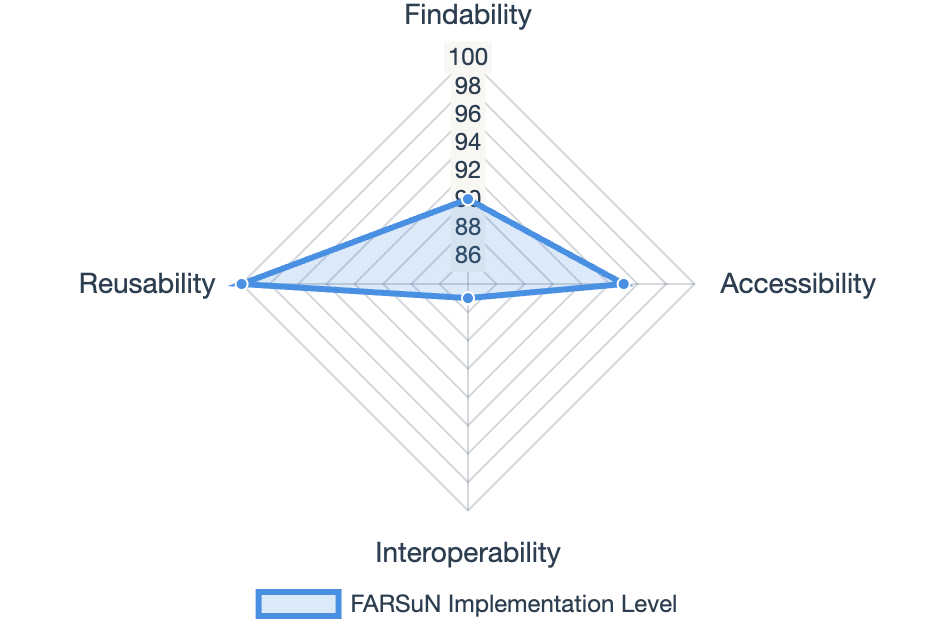
\includegraphics[width=\linewidth]{../figures/fair_radar.png}
% \end{tightblock}
\begin{tightblock}{FARSuN Historical Sunspot Database} % — Status \& Outlook}
  A sustainable, interoperable reference database ensuring that four centuries of solar observations remain accessible and scientifically reliable for the next generation of Sun-climate research. 
  % \textbf{Present Status}
  \begin{itemize}
    \item Legacy sources (Mitteilungen, Wolf Institute, Shreya, Stephen, etc.) have been integrated into the current schema for cross-validation and QC.
    \item Automated quality checks detect inconsistencies (e.g., NG $>$ NS, duplicates, missing metadata).
    \item Metadata harmonization for observers, instruments, and observatories is underway.%, aligned with the EPN-TAP/VO standard for public access.
    % \item A TAP server at ROB is operational, enabling ADQL queries and VOTable outputs.
  \end{itemize}

  \textbf{Next Steps}
  \begin{itemize}
    \item Finalize canonical schema and close remaining legacy mappings.
    \item Expand automated QC dashboards and uncertainty modeling.
    \item Scale up digitization and extraction (Adams, Gruithuisen, Stark, etc.) using HTR and citizen-science workflows.
    \item Expose the full dataset through the EPN-TAP service, ensuring FAIR data availability.
    \item Use this harmonized database as the foundation for $S_{N}$ V3.0 calibration and long-term solar activity studies.
  \end{itemize}

\end{tightblock}

\begin{tightblock}{Methods}
\begin{itemize}
  \item Dual-mode transcription: tailored Transkribus handwriting models plus manual keying for complex tables.
  \item Data hygiene: observer alias reconciliation, calendar conversions, and spot/group recount audits.
  \item Uncertainty modelling: propagate observer calibration curves and note spotless-day confidence flags.
  \item Automation: reproducible Python pipelines with checkpoints for citizen-science ingestion and review.
\end{itemize}
\end{tightblock}

\begin{tightblock}{Quality Gates}
\begin{itemize}
  \item Two-person verification for Adams and Gruithuisen counts before publishing derived indices.
  \item Cross-compare FARSuN transcriptions with Wolf's \emph{Mittheilungen} and modern SILSO indices for drift detection.
  \item Metadata harmonisation ensures unique observer IDs, instrument notes, and weather context survive downstream.
  \item Git-tracked pipelines and notebooks capture every transformation for audit and reuse.
\end{itemize}
\end{tightblock}

\end{column}


% -------- COLUMN 2 --------
\begin{column}{0.42\paperwidth}
\begin{tightblock}{Key Datasets}
\vspace{ 0.4em}
  \datasetbox{Mittheilungen Dataset (1610--1945)}{codegreen}
\vspace{ 0.4em}

% \textbf{Next steps}
% \begin{itemize}
%   \item Full public release via Virtual Observatory access.
%   \item Inclusion of Mittheilungen as the core calibration reference for $S_{N}$ Version 3.
%   \item Development of interactive QC dashboards and documentation to support open, traceable historical solar research.
% \end{itemize}
\begin{figure}[t]
  \centering
  \begin{minipage}[t]{0.45\linewidth}
    \vspace{0pt}
    The Mittheilungen journals, compiled by Rudolf Wolf and successors at the Zürich Observatory, form a central source of historical sunspot observations. They document daily group and spot counts from 1848 to 1945 and incorporate earlier material back to 1610 through Wolf’s compilations. Within the FARSuN project, the complete series was digitized and structured at the Royal Observatory of Belgium, integrated into the historical sunspot database, and is undergoing continued quality checks, metadata harmonization, and cross-comparisons with newly recovered records. This digitized dataset now provides four centuries of observer statistics and constitutes a key component of the historical foundation for the ongoing reconstruction of $S_{N}$ V3.0.

%     The Mittheilungen journals, compiled by Rudolf Wolf and successors at the Zürich Observatory, form a central source of historical sunspot observations, documenting daily group and spot counts from 1848 to 1945 and incorporating earlier material back to 1610 through Wolf’s compilations. Within the FARSuN project, the full series was digitized and structured at the Royal Observatory of Belgium, integrated into the historical sunspot database, and is now undergoing continued quality checks, metadata harmonization, and cross-comparisons with newly recovered records.
%
% % The Mittheilungen journals, compiled by Rudolf Wolf and successors at the Zürich Observatory, form the backbone of historical sunspot observations, recording daily group and spot counts from 1848 to 1945 and extending back to 1610 through Wolf's compilations.%; within the FARSuN project, the complete series was digitized and structured (2017--2019) at the Royal Observatory of Belgium, integrated into the historical sunspot database, and is undergoing continuing quality checks, metadata harmonization, and cross-comparisons with new extractions.
% They are now fully digitized and integrated in FARSuN, providing four centuries of observer statistics and forming a key component of the historical foundation needed for the ongoing reconstruction of $S_{N}$ V3.0.
%
% % \textbf{Current focus}
\begin{itemize}
  \item Refining data consistency and observer calibration (Wolf--Wolfer overlap).
  \item Finalizing metadata alignment for FAIR publication. 
  \item Resolving remaining ID and provenance issues across merged databases.
\end{itemize}
    % \centering
    % 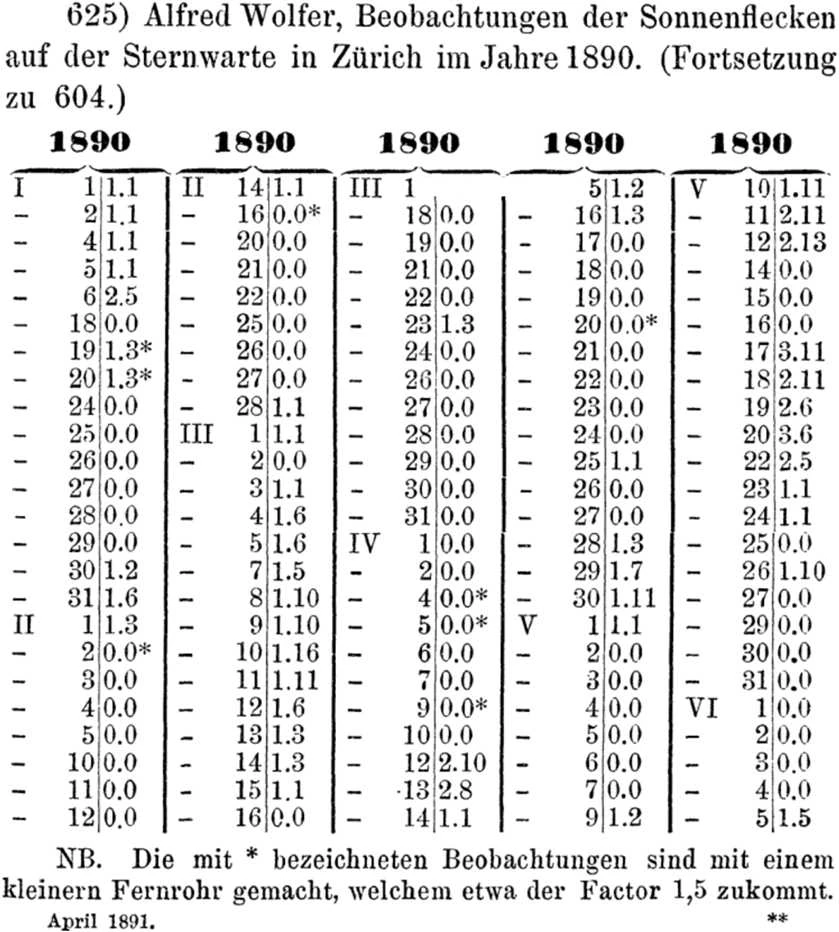
\includegraphics[width=\linewidth]{../figures/mittheilungen_sample.png}
    % {\small (a) Typical yearly table(in the Mittheilungen)}
    % {(first page going up to early June). The table lists all daily observations from A.~Wolfer for 1890 with group and spot totals separated by a dot; stars mark days observed with a 40\,mm ``Parisian'' telescope.}
  \end{minipage}
  \hfill
  \begin{minipage}[t]{0.52\linewidth}
    \vspace{0pt}
    \centering
    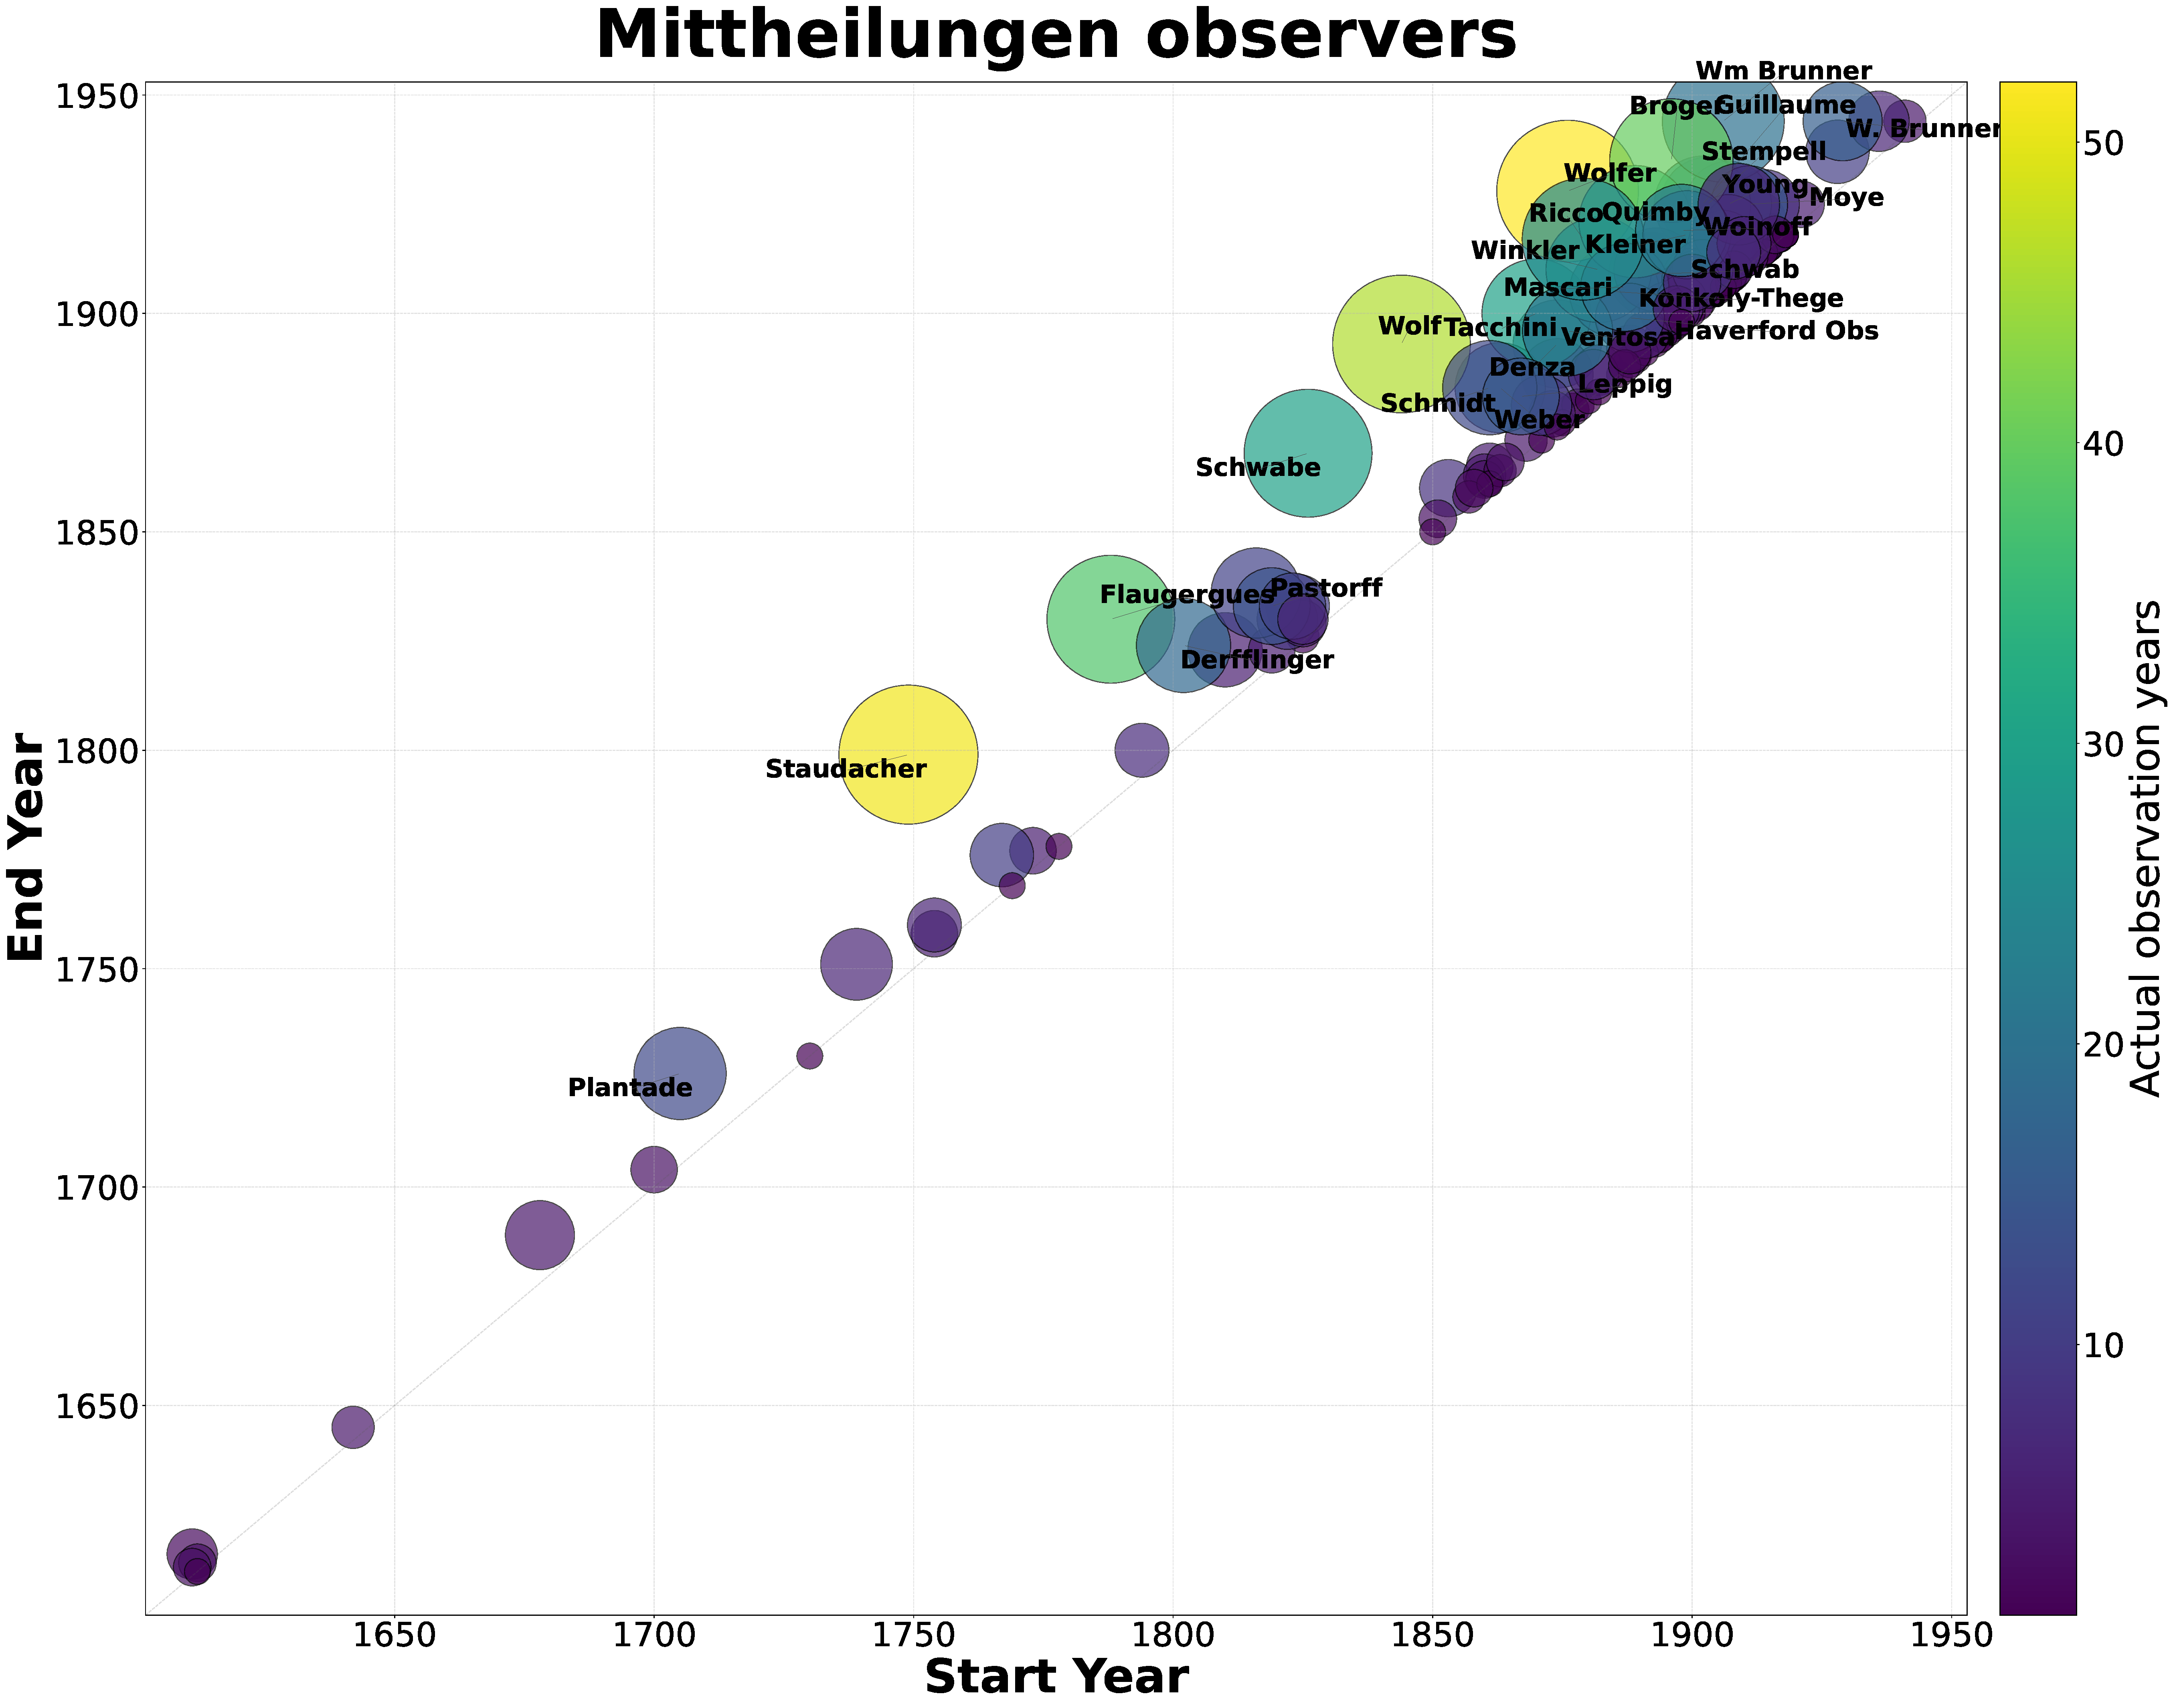
\includegraphics[width=\linewidth]{../figures/mitt_observer_bubble.pdf}
    % {\small (b) Observer coverage and overlaps}% that anchor cross-calibration.}
  \end{minipage}
  % \caption{\small Mittheilungen facsimile (a) and observer coverage overview (b) illustrating the documentation pipeline that links historical records to calibrated metadata.}
\end{figure}
\vspace{-01.4em}
\datasetbox{Z\"urich Tables (1945--1979)}{codeblue}
% \begin{minipage}[t]{0.3\linewidth}
  \vspace{0.2cm}
The Z\"urich Tables form the foundational record of daily sunspot number production at the Z\"urich Observatory between 1945 and 1979, detailing group and spot counts, the adopted Wolf number, and observing context.
\textit{Status}: 95\% of the 2\,000+ yearly tables are already digitized and the remaining late-1970s observer metadata are being encoded.
\vspace{0.3em}
% \textbf{Current status}
\begin{itemize}
  \item Fully digitized for 1945--1979 with detailed metadata completed for 1945--1959.
  \item Quality control and observer metadata harmonisation underway to maintain traceability.
  % \item Integration to consolidated FARSuN database is underway.
\end{itemize}
% \hfill
% \end{minipage}
% \begin{minipage}[t]{0.7\linewidth}
%   \vspace{0pt}
% % \textbf{Next steps}
% % \begin{itemize}
% %   \item Complete metadata for later years, confirm 1980 holdings, and refine observer scaling (k-factors).
% %   \item Analyse the 1947 scale discontinuity and publish cleaned, validated releases linked with USET drawings.
% %   \item Deliver public access to the curated Z\"urich dataset to support reconstruction of $S_{N}$~V3.0.
% % \end{itemize}
%   \centering
%   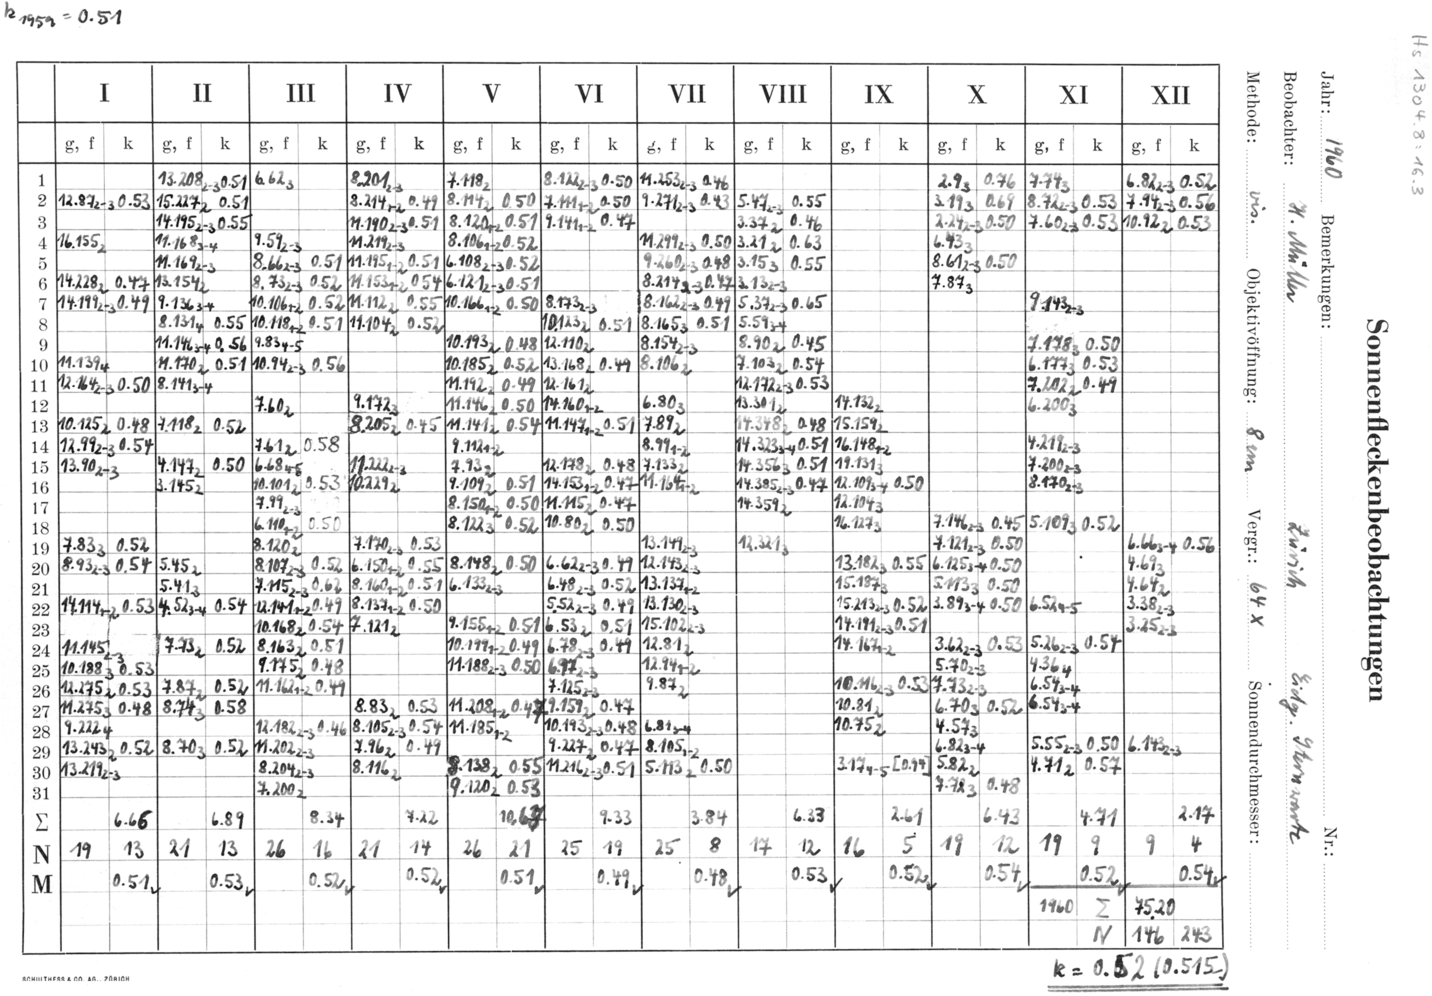
\includegraphics[width=\linewidth]{../figures/zurich_tables.png}\\[0.3em]
%   {\small Facsimile of a typical handwritten yearly table}% from the complete 1945--1980 collection recovered in 2018--2019. Shown are H.~M\"uller's 1960 observations with group totals, spot counts, personal $k$ relative to Waldmeier, sky quality, monthly aggregates, and yearly averages, highlighting assistant-to-primary dispersion (here $k=0.52$ versus the 0.6 target).}
% \end{minipage}

\datasetbox{Gruithuisen Data (1817--1849)}{codeorange}% — Present Status \& Future
\vspace{0.3em}
The Gruithuisen manuscripts (1817--1849) capture daily sunspot notes, drawings, and weather context in German Kurrent script, supplying early-19th-century coverage vital for $S_{N}$~V3.0 refinement.
The entire image set is digitized and extraction via bespoke Transkribus-style models plus dual QC for NG/NS tallies is underway.

% \textbf{Present status (Oct 2025)}
\begin{itemize}
  \item Image sets and text snippets fully collected with preliminary CSV/XLSX extraction completed.
  \item Two-pass QC (survey + counting) with verified sunspot counts in progress.
\end{itemize}

% \textbf{Next steps}
% \begin{itemize}
%   \item Finalise daily presence/absence and NG/NS values, and complete dual QC plus metadata registry.
%   \item Calibrate with coeval observers to stabilise scaling.
%   \item Publish FAIR, VO-ready daily tables and image catalogues via ROB/SILSO to support $S_{N}$~V3.0 calibration and uncertainty modelling.
% \end{itemize}
\begin{figure}[t]
  \centering
  \begin{minipage}[t]{0.50\linewidth}
    \centering
    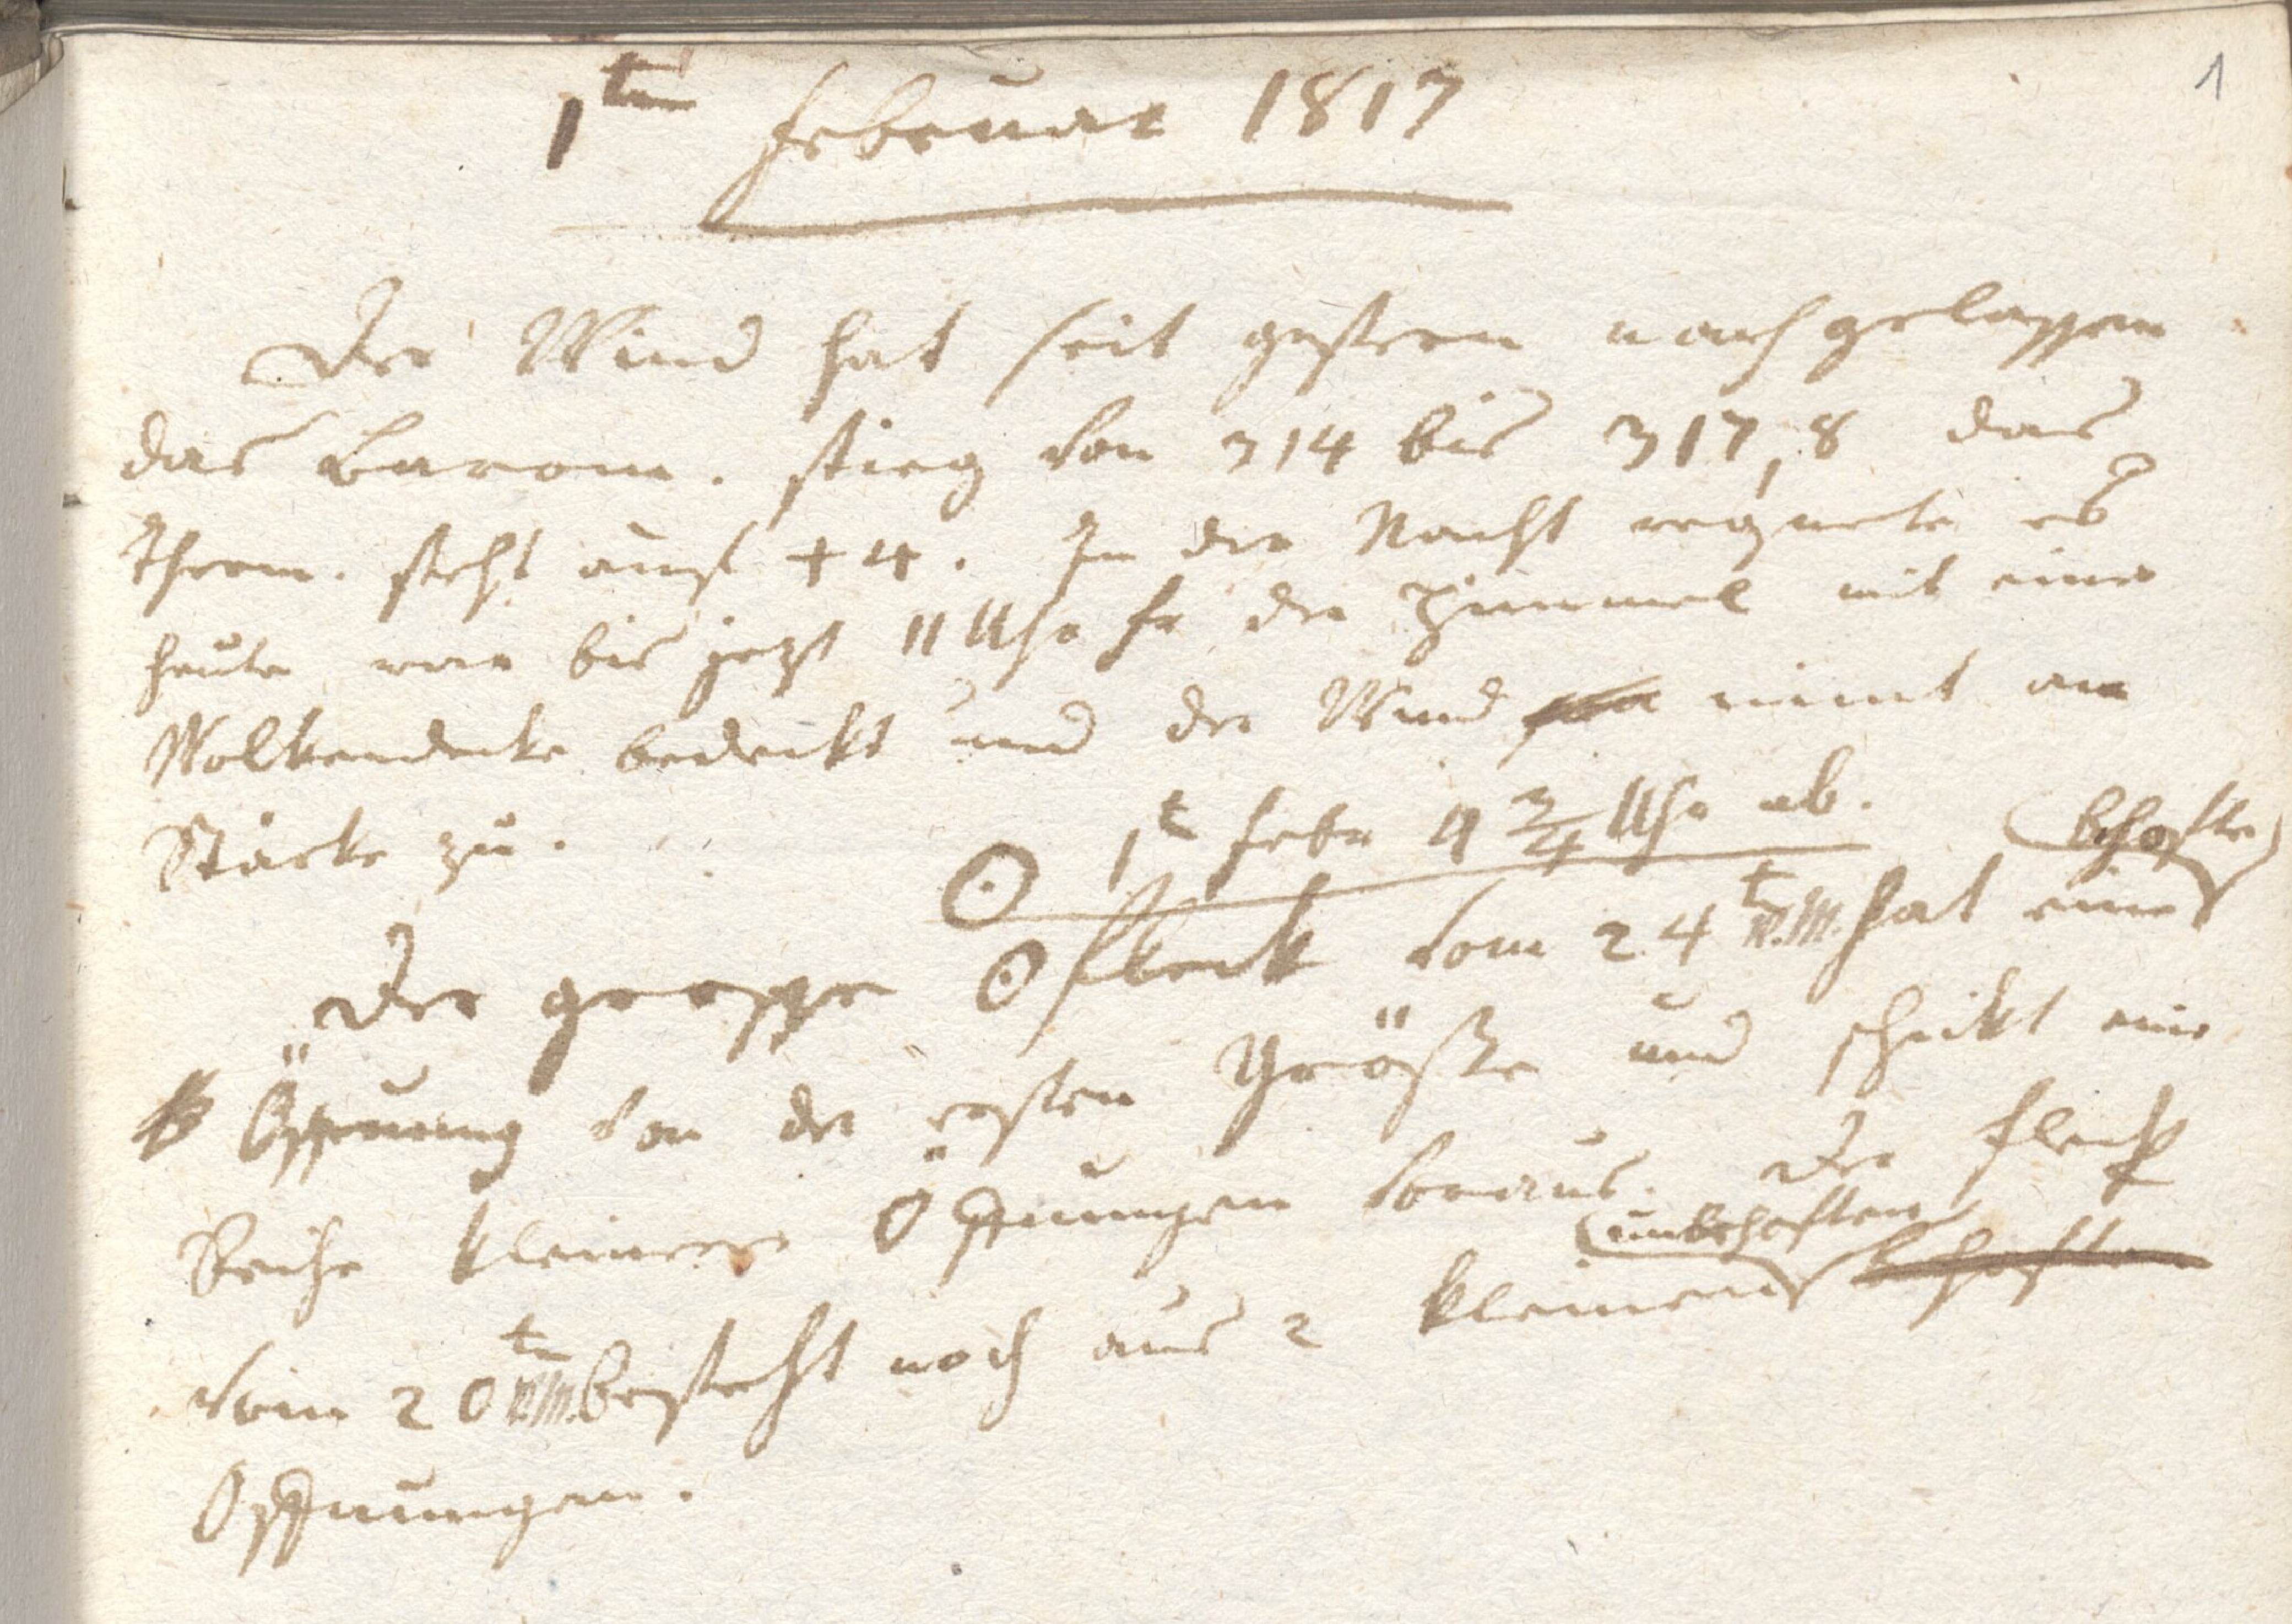
\includegraphics[width=\linewidth]{../figures/Gruithuisen_Sample1.png}
    % {\small (a) Daily log highlighting spotless spans and sky notes.}
  \end{minipage}\hfill
  \begin{minipage}[t]{0.47\linewidth}
    \centering
    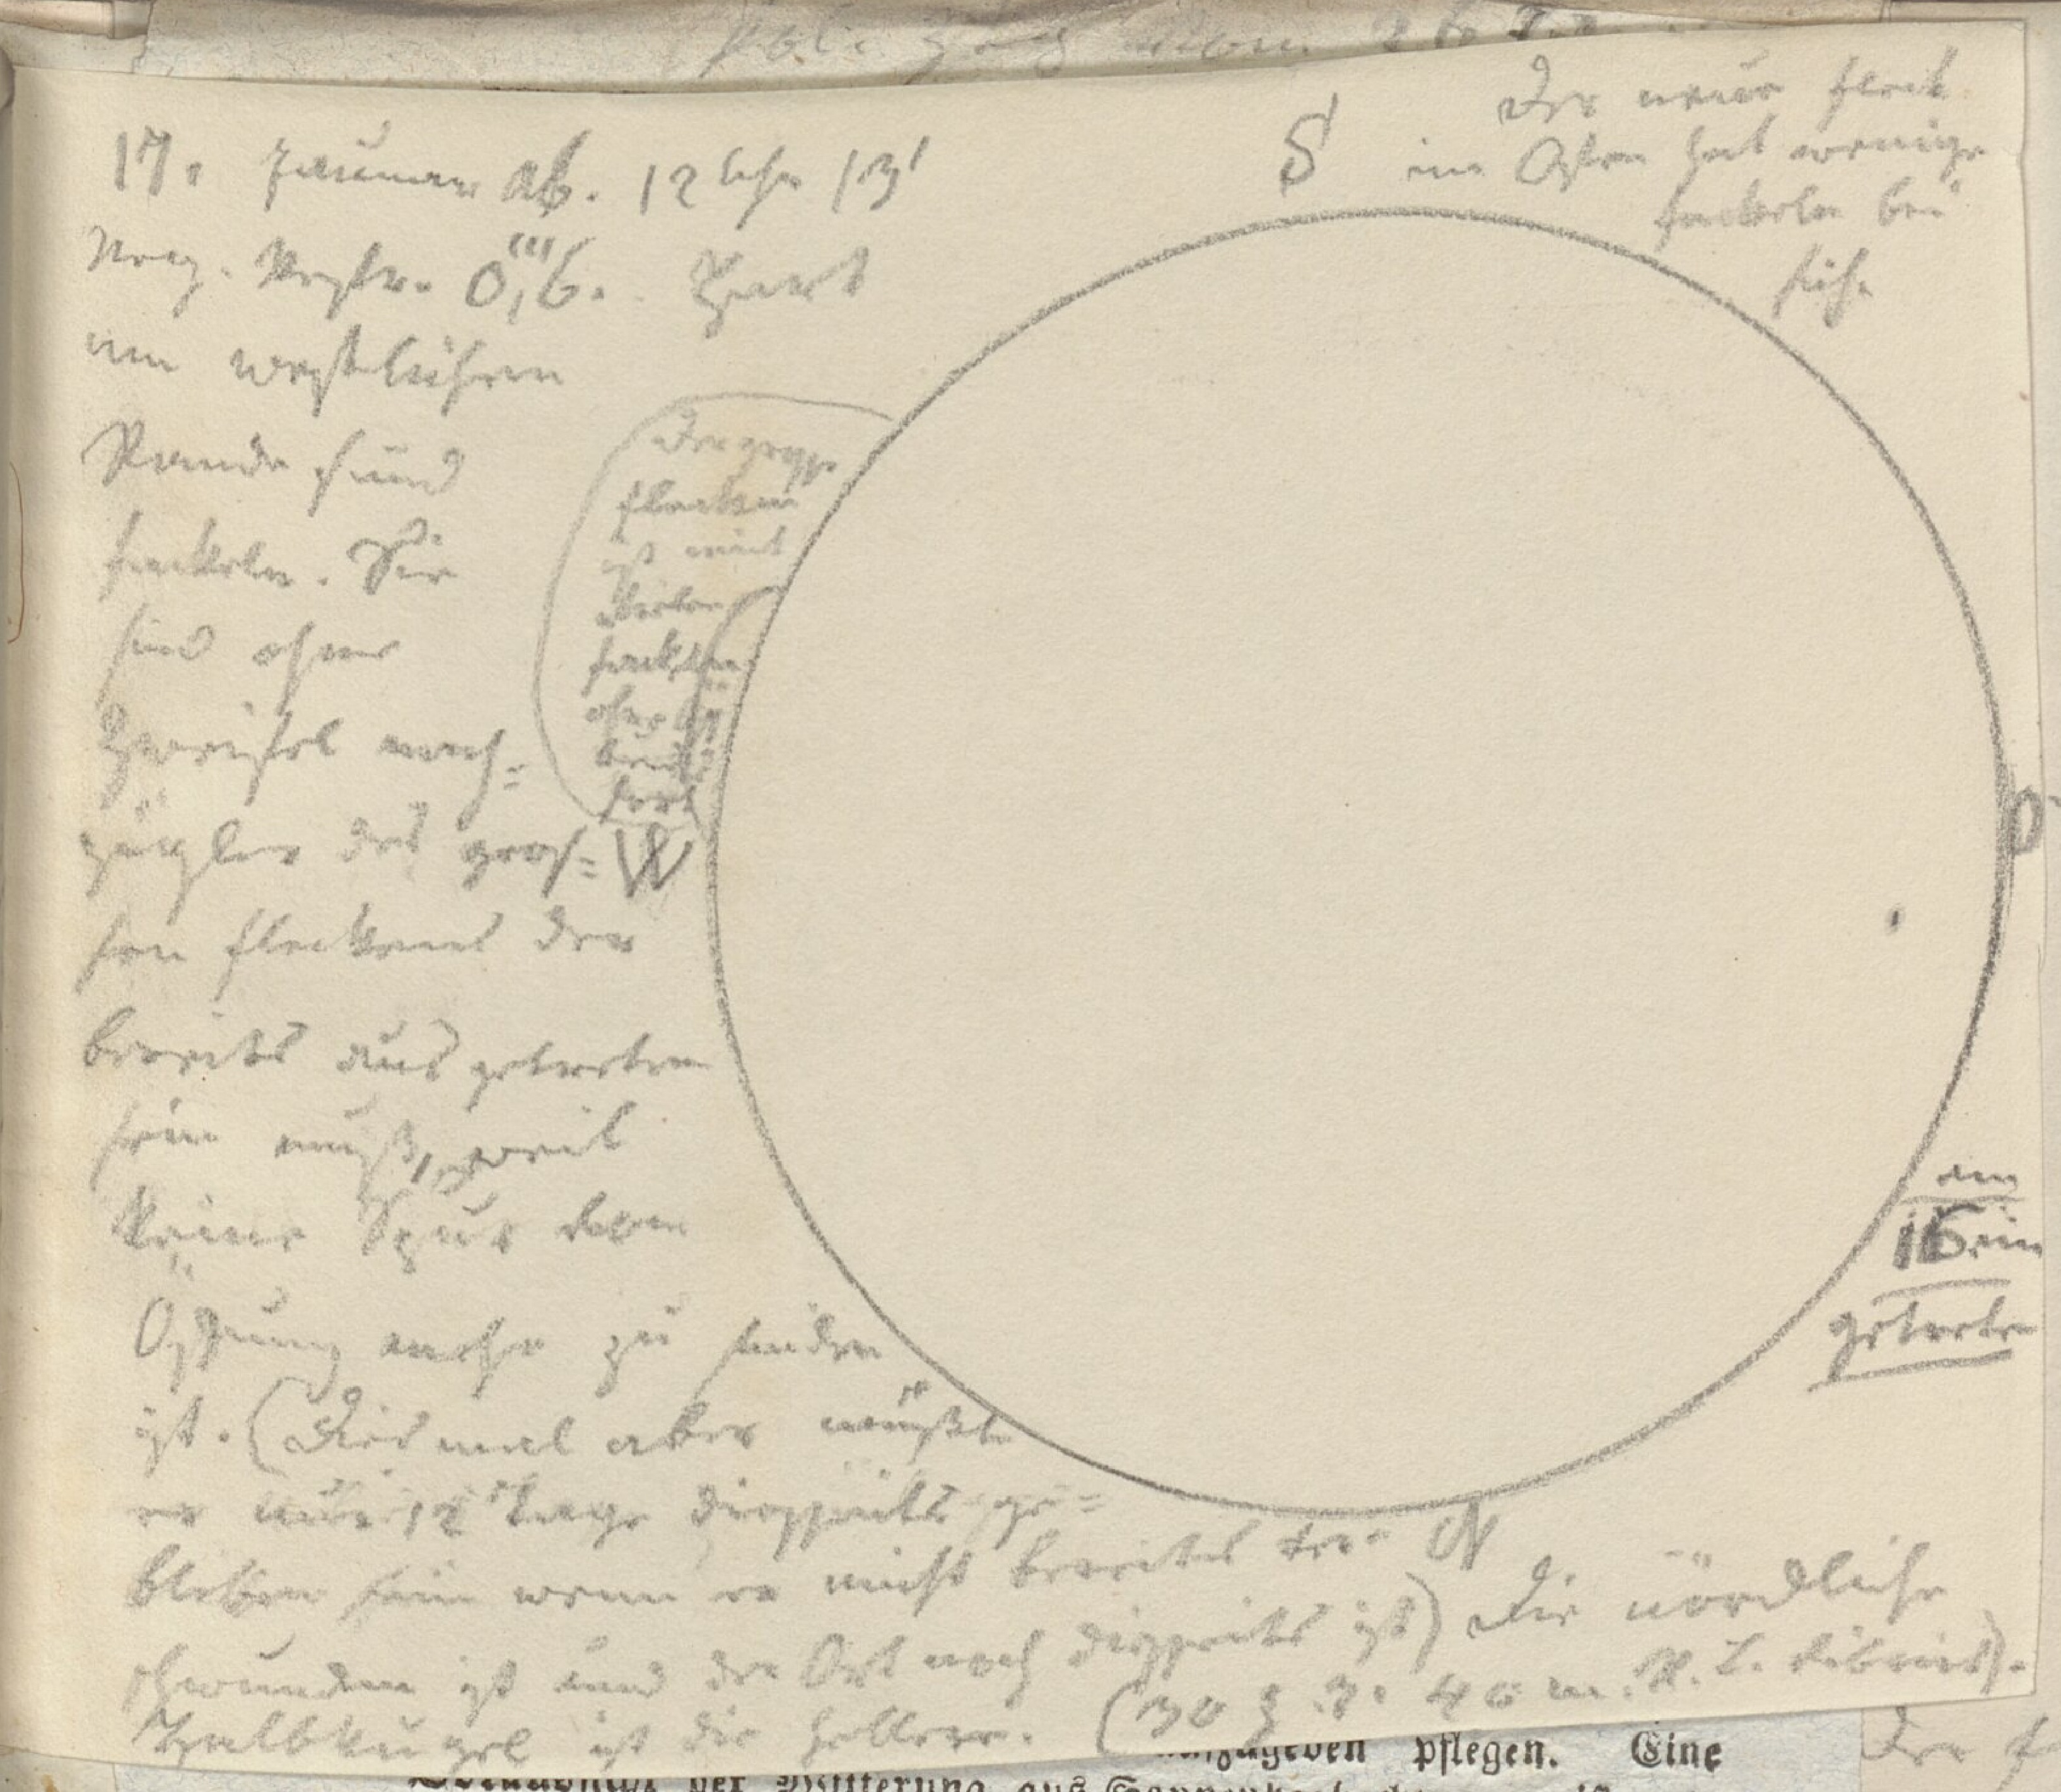
\includegraphics[width=\linewidth]{../figures/Gruithuisen_Sample2.jpg}
    % {\small (b) Extract with NG/NS tallies and observer annotations.}
  \end{minipage}
\end{figure}

\vspace{0.5em}
  \datasetbox{C.~H. Adams Data (1819--1823)}{codepurple} % — Present Status \& Future Work
\vspace{0.3em}
FARSuN has recovered 338 full-disk drawings and 1,056 daily entries (308 spot days, 748 spotless) from C.~H.~Adams (1819--1823), providing dense coverage with explicit spotless days.
All spotless-day tallies are cross-checked against Wolf's compilations, anchoring early-1800s calibration experiments.

% \vspace{0.3em}
% \textbf{Current work}
\begin{itemize}
  \item Quality checks to align direct and reflection methods for consistent calibration.  
  % \item Cross-check with Mittheilungen and other contemporaneous observers.
  \item Orientation, and standardisation of drawings to enable future positional and area extractions.
\end{itemize}
% \begin{figure}[t]
%   \centering
% 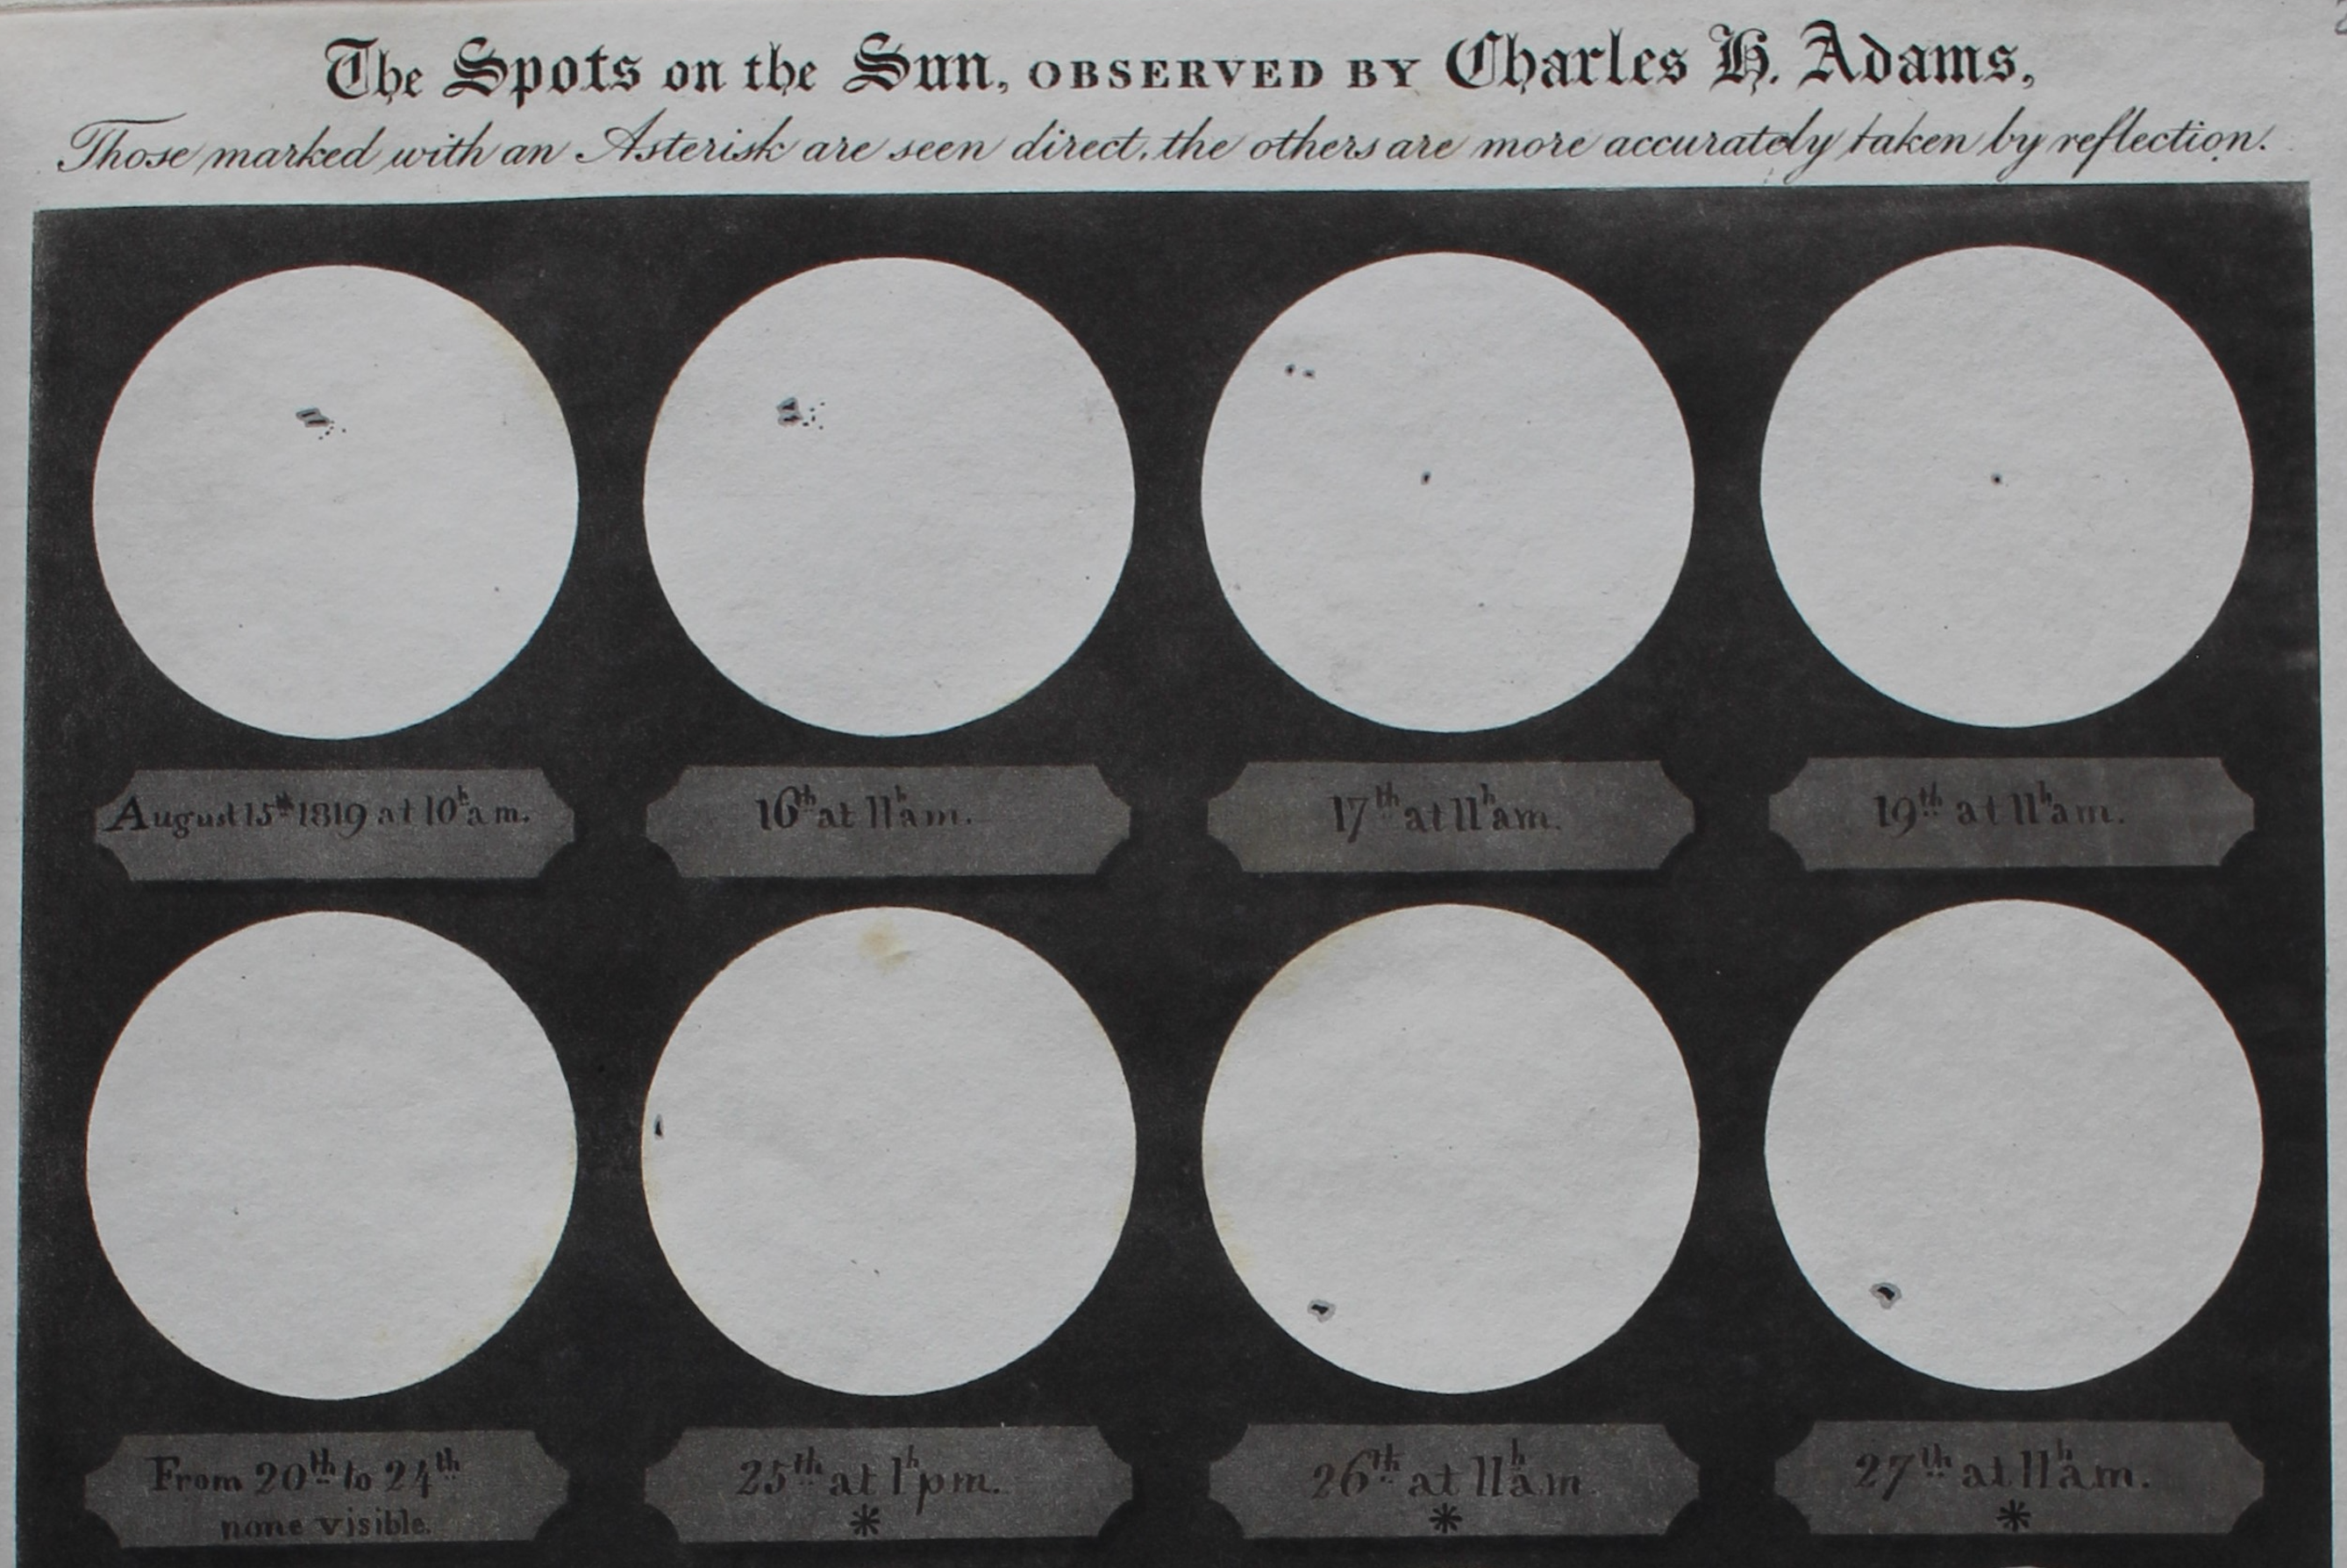
\includegraphics[width=0.65\linewidth]{../figures/adams_example.png}
% \end{figure}
% \\


\end{tightblock}

\end{column}

% -------- COLUMN 3 --------
\begin{column}{0.26\paperwidth}
{\small
\begin{tightblock}{Key Datasets}
\datasetbox{Augustin Stark Data (1813--1835)}{codered}
{
The Stark dataset (1813--1835), comprising printed German descriptions of sunspot groups and chains, has been partially retrieved. Preliminary OCR and extraction tests show good potential, and ongoing work focuses on refining consistency, QC flags, and metadata integration into the FARSuN database. Trial extraction campaigns continue so that descriptive passages are tagged consistently before bulk ingestion.
}
\datasetbox{Data Recovery Efforts Since 2010}{codecomment}
{
  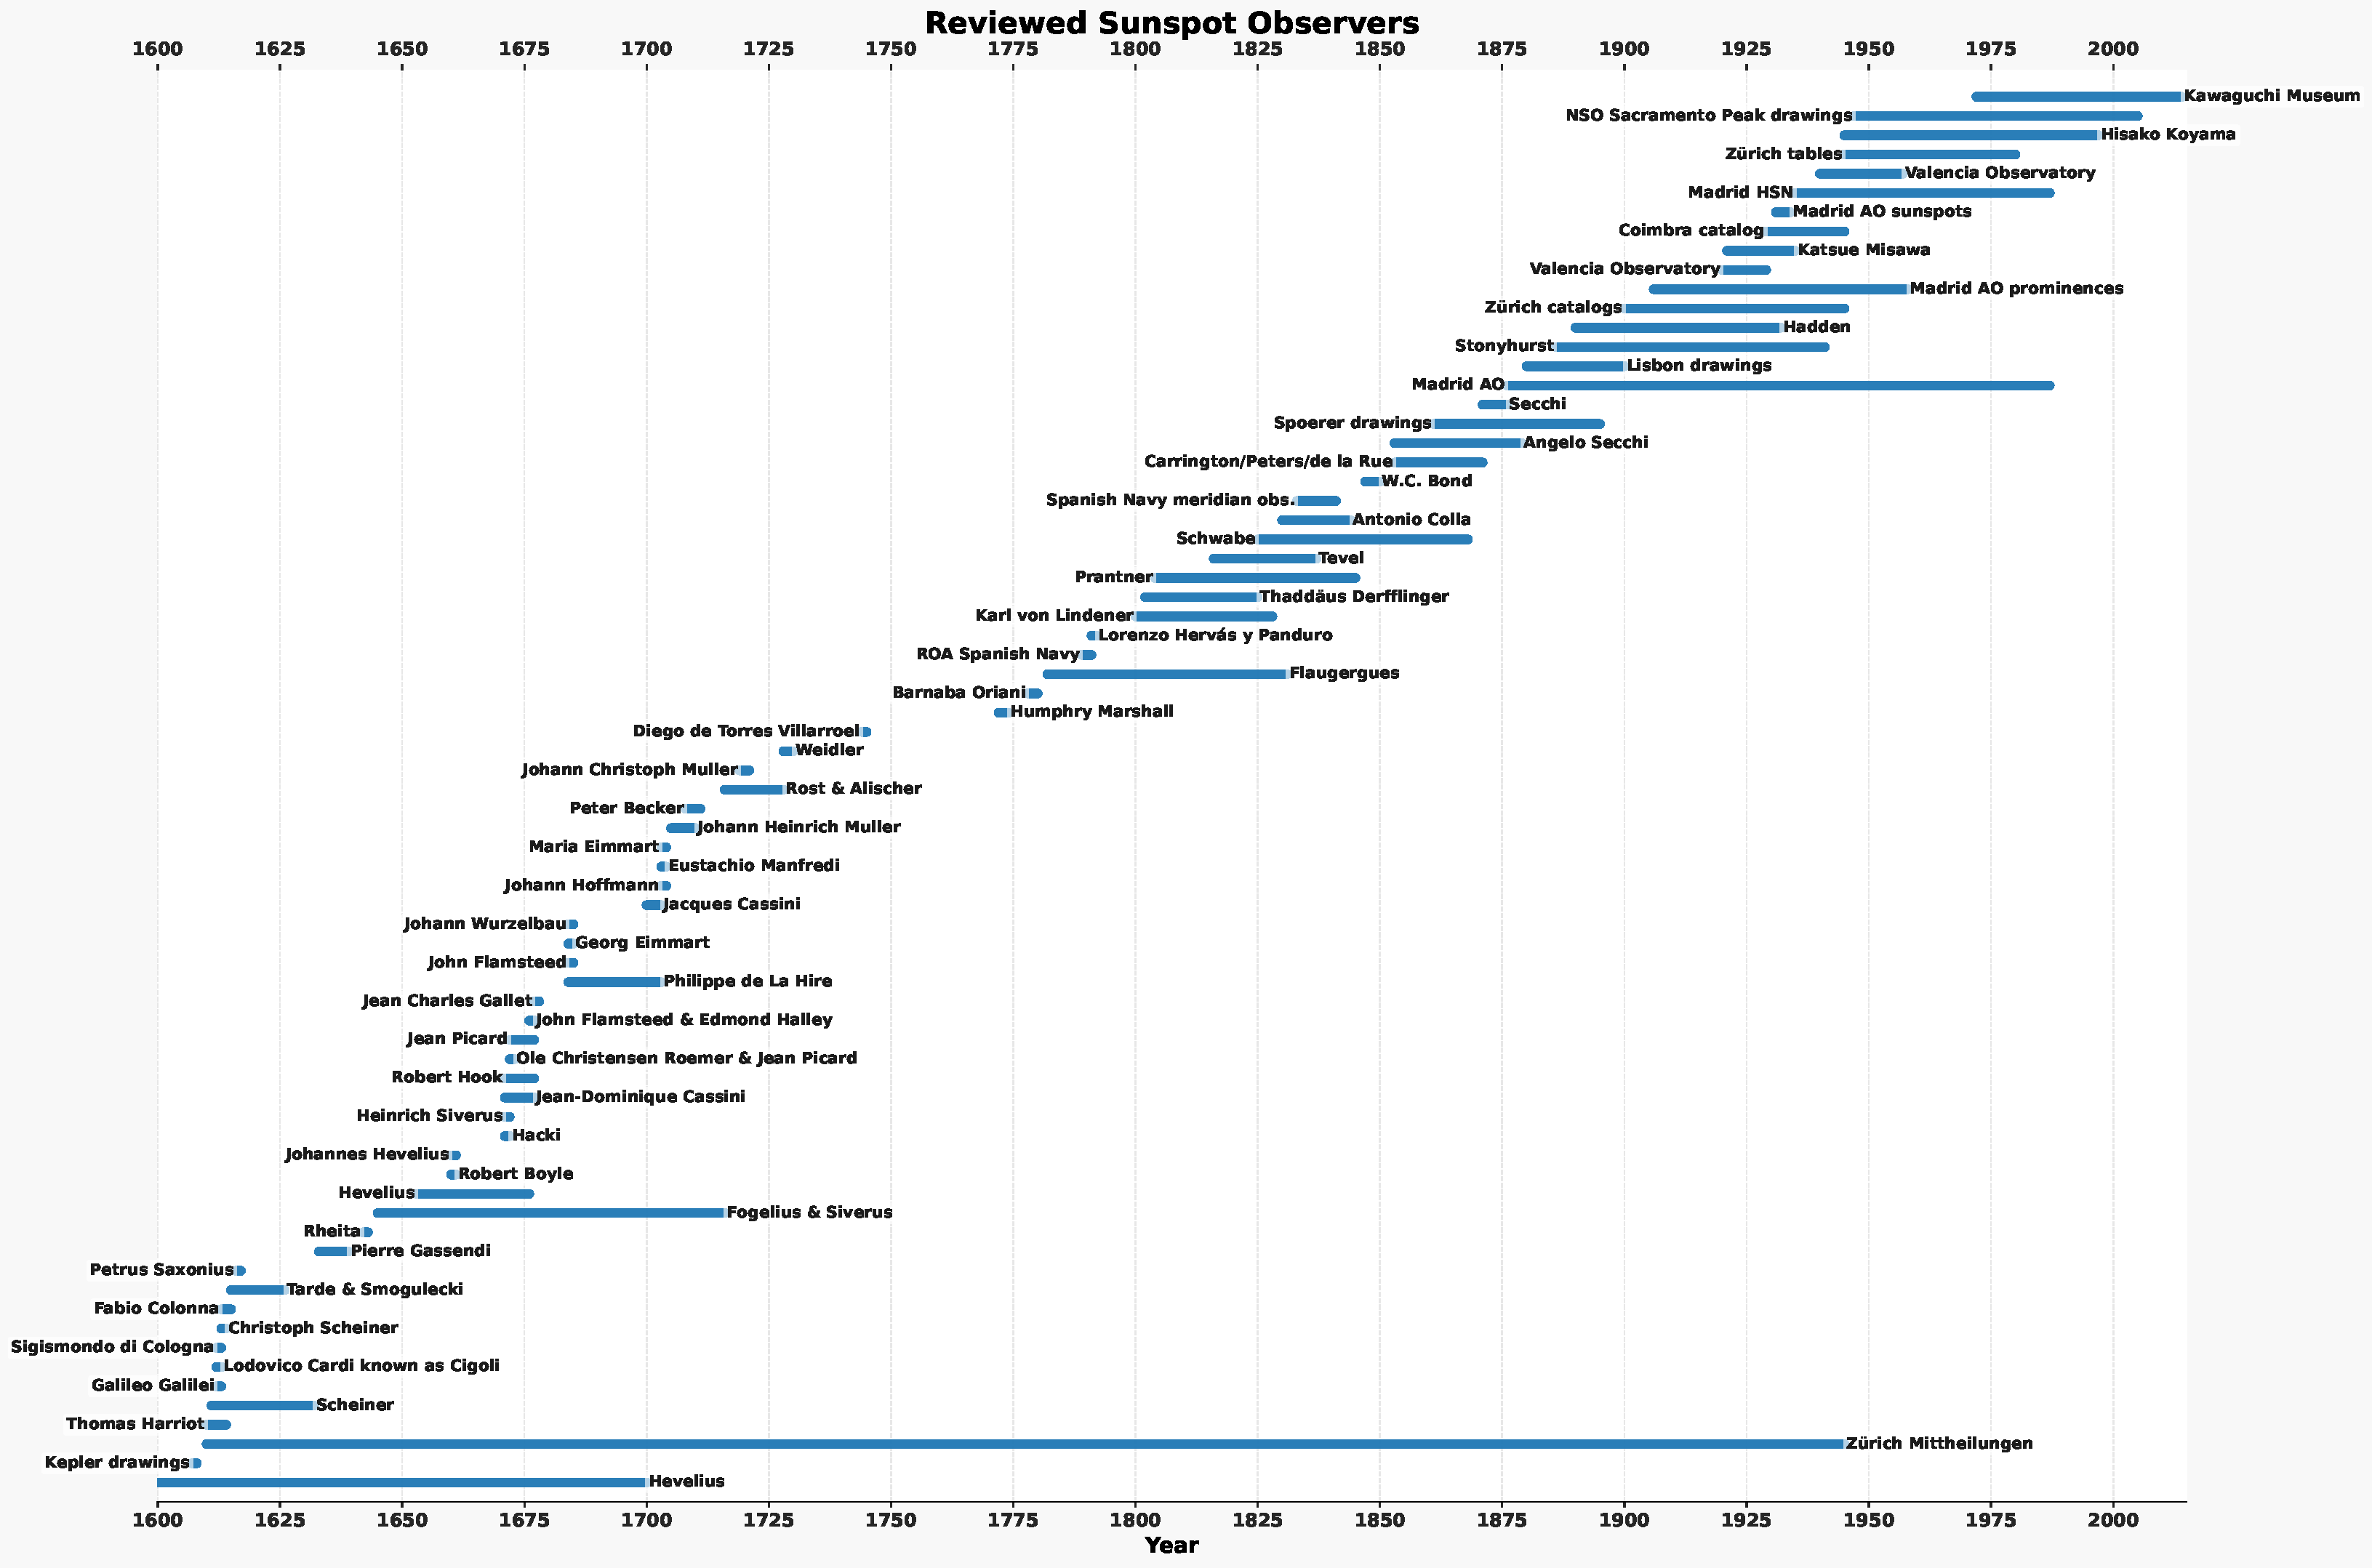
\includegraphics[width=\linewidth]{../figures/reviewed_sources_timeline_merged.pdf}
A non-exhaustive set of early telescopic sunspot datasets recovered and published since 2010, showing their temporal coverage from the early 1600s to the modern era. These community efforts—including major contributions by Hayakawa, Arlt, Vaquero, Carrasco, and others—have greatly expanded the number of available raw observations, enabling independent cross-checks of overlapping observers.
}
\end{tightblock}
\begin{tightblock}{Progress Highlights}
\begin{itemize}
  \item Citizen-science interface blueprint prepared for the upcoming transcription portal.
  \item Z\"urich pipeline combines Transkribus extraction with manual review to reach the 2026 target.
  \item Gruithuisen workflow couples Kurrent experts with validation scripts to catch missing symbols.
  \item Adams drawings cross-checked with \emph{Mittheilungen} records to confirm spotless-day agreement.
\end{itemize}
\end{tightblock}

\begin{tightblock}{Challenges}
\begin{itemize}
  \item Deciphering \emph{Kurrent} manuscripts and annotating non-solar notes without losing context.
  \item Harmonising heterogeneous formats (drawings, tabular ledgers, weather marginalia).
  \item Quantifying observer bias and spotless-day reporting habits over centuries.
  \item Maintaining end-to-end provenance from scanned folio to released data product.
\end{itemize}
\end{tightblock}

\begin{tightblock}{From Raw to $S_{N}$ V3.0}
\begin{enumerate}
  \item Curate daily counts with provenance-rich metadata (observer, instrument, weather context).
  \item Solve observer response functions to align group/spot scales across centuries.
  \item Aggregate to monthly, yearly, and hemispheric indices with propagated uncertainties.
  \item Benchmark against $S_{N}$~V2.0 and satellite-era proxies to validate drift corrections.
\end{enumerate}
% 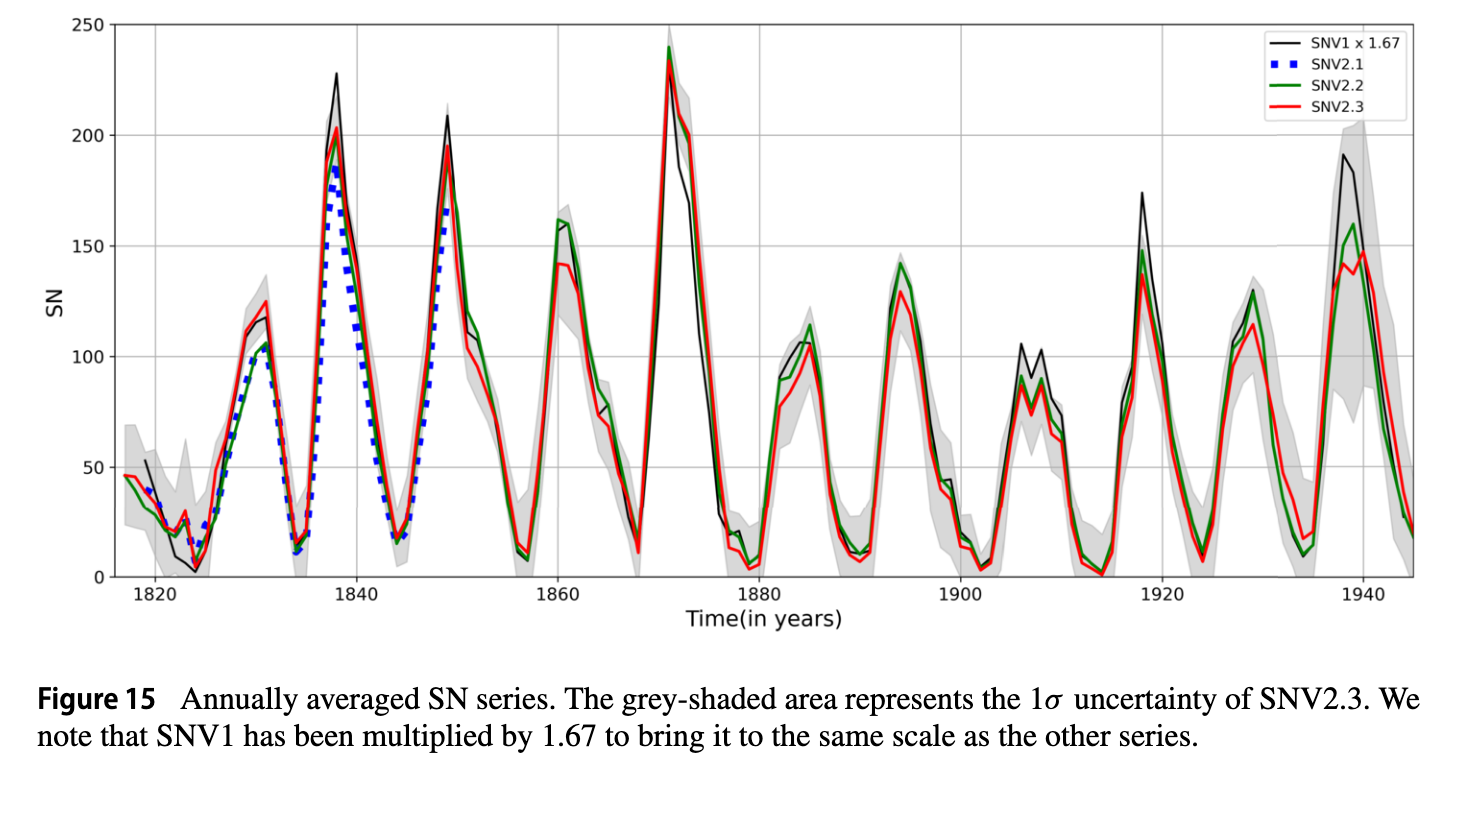
\includegraphics[width=0.9\linewidth]{../figures/comparison_panel.png}
\end{tightblock}

\begin{tightblock}{Space Climate Impact}
\begin{minipage}[t]{0.48\linewidth}
  \callout{\color{codestring}Citizen science}{Interactive portal mobilises volunteers to transcribe \emph{Kurrent} manuscripts and sustain STEM outreach.}
\end{minipage}\hfill
\begin{minipage}[t]{0.48\linewidth}
  \callout{\color{codeblue}Forecasting}{Bias-free $S_{N}$~V3.0 improves solar cycle prediction skill and operational space weather baselines.}
\end{minipage}
\par\vspace{0.25em}
\begin{minipage}[t]{0.48\linewidth}
  \callout{\color{codeorange}Climate links}{Validated historical forcing refines long-term climate models and Earth radiation budget studies.}
\end{minipage}\hfill
\begin{minipage}[t]{0.48\linewidth}
  \callout{\color{codegreen}Open science}{FAIR-compliant releases with APIs and uncertainty bundles accelerate community reuse.}
\end{minipage}
\end{tightblock}




\begin{tightblock}{Poster QR Code}
\begin{figure}[t]
  % \centering
  % \begin{minipage}[t]{0.70\linewidth}
 For more information on FARSuN project, datasets, and a digital copy of the poster, scan the QR code.
  % \end{minipage}
  \hfill

  \begin{minipage}[t]{0.25\linewidth}
    \centering
    
\includegraphics[width=\linewidth]{../docs/figures/qrcode_farsun-poster.png}
    % \par\vspace{0.2em}
    % \vspace{-0.3em}
  \end{minipage}
\end{figure}
\end{tightblock}

% \begin{tightblock}{Outlook}
% \begin{itemize}
%   \item Launch the citizen-science transcription portal with targeted training.
%   \item Publish $S_{N}$~V3.0 release notes covering uncertainties and API endpoints.
%   \item Broaden partnerships (Nagoya, UCLouvain, ROB) for cross-validation and joint papers.
% \end{itemize}
% \end{tightblock}

\vspace{-0.5em}
\par}
\end{column}

\end{columns}
\end{frame}
\end{document}
